% this package changes the paragraph style to skip a line before a new paragraph rather than indenting% font size
\documentclass[11pt]{article}
\usepackage{fullpage,parskip,amsmath,amssymb,algorithm2e,enumitem,graphicx}
\usepackage{hyperref}
\usepackage{graphicx}
\usepackage{wrapfig}
\usepackage{array}

\hypersetup{
    colorlinks=true,
    linkcolor=blue,
    filecolor=magenta,      
    urlcolor=blue,
    pdftitle={Overleaf Example},
    pdfpagemode=FullScreen,
    }
\usepackage{xcolor}

\parindent24pt
\pagestyle{empty}

\newcommand{\n}{\newcommand%
}
\renewcommand{\r}{\renewcommand%
}
\SetAlgoLined
\r{\bf}{\textbf}
\r{\it}{\textit}
\n{\ol}{\overline}
\n{\ul}{\underline}
\n{\unspace}{\vspace{-2.15em}}
\AtBeginEnvironment{align}{\setcounter{equation}{0}\vspace{-18pt}}
\AtBeginEnvironment{flalign}{\setcounter{equation}{0}}
\AtBeginEnvironment{align}{\unspace}
\AtBeginEnvironment{align*}{\unspace}
\AtBeginEnvironment{flalign}{\unspace}
\AtBeginEnvironment{flalign*}{\unspace}
\AtBeginEnvironment{algorithm}{\Indp}
\setenumerate[1]{label=\bf{(\arabic*)}}
\n{\note}[1]{\it{Note: }#1}
\newenvironment{proof}[1]{\it{pf: }This is a proof by #1.\par \begin{itemize}}{\end{itemize}}
\SetKwBlock{Blk}{}{}
\n{\Fn}[3]{\KwSty{Function} \ArgSty{#1(#2)}\Blk{#3}}


\begin{document}

\noindent\boxed{
\begin{tabular*}{\textwidth}{@{}l@{\extracolsep{\fill}}r@{}}
CSCI 2600 --- Principles of Software\\\\
\multicolumn{2}{c}{\huge{Homework 7: Model-View-Controller and RPI Campus Paths}}\\
\multicolumn{2}{c}{\it{Due: Wednesday, April 26, 2023,  11:59:59 pm}}\\\\
\end{tabular*}}
\par


\noindent {\huge\textbf{\underline{Submission Instructions}}}
\begin{itemize}
\item  
This assignment uses the same repository as Homework assignments 4, 5, and 6, so when you are ready to start working on Homework 7, pull Homework 7 files from the repository by right-clicking on your Homework 4 project in Eclipse and selecting \texttt{Team -$>$ Pull...} Make sure that \texttt{When pulling} is set to \texttt{Merge}, then click \texttt{Finish}.

\item
Be sure to commit and push the files to Submitty. Follow the directions in the \href{https://www.cs.rpi.edu/academics/courses/spring23/csci2600/Documents/eclipse_and_git.pdf}{version control handout} for adding and committing files.

\item
Be sure to add any additional files to your repo using Team/Add to Index.

\item
\textcolor{red}{\textbf{Important:} You must press the \textbf{Grade My Repository} button, or your answers will not be graded.}
\end{itemize}

\noindent {\huge\textbf{\underline{IMPORTANT NOTES:}}}
\newline

\noindent You should have package 
\texttt{hw7} with the usual directory structure. Write your code under \texttt{src/main/java/hw7} and your tests under \texttt{src/test/java/hw7} (shows as \texttt{hw7} under \texttt{src/test/java} in Package Explorer). If your directory structure is incorrect autograding will fail resulting in a grade of 0!

\noindent {\huge\textbf{\underline{Introduction}}}
\newline

\noindent You will be building a route-finding tool. It will take the names or ids of two buildings on the RPI Troy Campus, and generate directions for the shortest route between them, using your graph ADT to represent buildings and pathways between them. For now you will provide a simple text interface. In this homework, you will write a complete application runnable from the command line via a \texttt{main} method. \textcolor{red}{You will have to name your main class CampusPaths.java for testing on the Homework Server.}

\noindent In this assignment, you will practice modular design, writing code for reuse, and design patterns. As before, you get to choose what classes to write and what data and methods each should have. Specifically, you will practice the model-view-controller (MVC) design pattern.

\noindent For organization, this assignment contains one "problem" for each logical component you will write. The order of the problems is not meant to suggest an order of implementation. \textbf{Carefully design} the whole system before attempting to implement any part. Design with "low coupling" and the "open/closed principle" in mind: you should be able to extend your system, while at the same time the heart of your system (your model) remains insulated from the changes. As always, you should develop incrementally, which may mean repeatedly writing a bit of all the parts and verifying that they work together.

\section*{Model-View-Controller}
\label{sec:MVC}

\noindent You will design your application according to the MVC design pattern described below. MVC is a variation of the Observer design pattern discussed in class.

\noindent As you design and implement your solution, please list which parts of your code belong to the model, the view, the controller, or none of the above in \texttt{answers/hw7\_mvc.pdf}. Often this can be on a per-class level, but when a class implements both the view and controller, you must indicate which methods or lines logically represent the view and which represent the controller. \textit{Be sure to list ALL classes you write for Homework 7.} This just should be a list of classes; you don't need to write any sentences of explanation.

\section*{The Three Pieces: Model, View, Controller}
\label{sec:The Three Pieces}

\begin{itemize}
\item The \textbf{model} consists of the classes that represent data, as well as the classes that load, store, look up, or operate on data. These classes know nothing about what information is displayed to the user and how it is formatted. Rather, the model exposes observer methods the view can call to get the information it needs.

In general, functionality of a model includes:
\begin{itemize}
\item Reading data from the data source (text file, database, etc.) to an in-memory representation.
\item Storing data while the program is running.
\item Providing methods for the view to access data.
\item Performing computations or operations involving the data and returning the result.
\item Updating the in-memory state (if the application allows the user to modify data).
\item Writing to the data source (text file, database, etc.)
\end{itemize}
\item The \textbf{view} implements the user interface. It should store as little data and perform as little computation as possible; instead, it should rely on the model for data storage and manipulation. The view decides how the user sees and interacts with these data.

Does the user interact with a text interface or a GUI? What does the user type and/or click to get directions from one building to another? How are those directions formatted for display? What message does the user see upon requesting directions to an unknown building? These are questions the view answers.

\item The \textbf{controller} listens to user input. Based on the user's keystrokes, mouse clicks, etc., the controller determines their intentions and dispatches to the appropriate methods in the model or view.
\textcolor{red}{For a simple interface like in this assignment, the view and controller may be somewhat intermingled in code. Don't worry too much about the separation there; the key point for now is that the model is cleanly separated and reusable.}
\end{itemize}

\section*{Model-View Interaction}
\label{sec:Model-View Interaction}

In general, avoid the temptation to create an oversized "god" class that does everything for the model. The model may contain multiple classes, and the view can interact with multiple classes in the model. Most of the time, any class that exists solely to represent data is part of the model. For this assignment, you will likely choose to have one central model class that manages the graph and does most of the heavy lifting, but you may also want some smaller objects that encapsulate related data. Some of these objects might be returned to the view so it can access their data directly, avoiding the "god" class scenario; others might only be used internally within the model.

\noindent Your model should be completely independent of the view (UI), which means it shouldn't know or decide how data is displayed. The model does know something about what data and operations the application needs, and it should provide methods to access them; however, it shouldn't return strings tailored to a particular view and definitely shouldn't contain \texttt{println}s. Imagine replacing your text UI with a GUI or a Spanish/Mandarin/Klingon text UI (but with the same English building names) and ask yourself: is my model reusable with this new view?

\noindent On the flip side, the view doesn't know anything about how the model stores data internally. Someone writing a view for your application should only know that the model somehow stores buildings and paths on campus and should only interact with the data at this level. In other words, the public interface of the model should give no indication that these data are represented internally as a graph. That level of detail is irrelevant to the view, and revealing it publicly means the model can no longer change its implementation without potentially breaking view code.

\section*{Problem 1: Parsing the Data}
\label{sec:Problem 1}

We have added two .csv data files to the \texttt{data/} directory to be parsed by your application: \texttt{RPI\_map\_data\_Nodes.csv} and \texttt{RPI\_map\_data\_Edges.csv}. The \texttt{.csv} files are comma-separated value files that can be opened in any text editor, just like \texttt{marvel.csv}. Their format is described in more detail below.

\noindent As usual, your program should look for files using filenames in your \texttt{data/} directory  e.g., 
\newline
\texttt{data/RPI\_map\_data\_Edges.csv}.

\noindent You will write a parser to load the data from these files into memory. You may use \texttt{MarvelParser.java} as a general example of how to read and parse a file, keeping in mind that the new data files are structured differently from the Marvel data file.

\noindent The file \texttt{RPI\_map\_data\_Nodes.csv} lists all buildings on campus along with their pixel coordinates on the campus map. (The image of the campus map can be downloaded here or a larger version from here).  File \texttt{RPI\_map\_data\_Nodes.csv} has two parts. The first part lists all the buildings on campus, where each line has four comma separated fields:

\noindent \texttt{Name,id,x-coordinate,y-coordinate}

\noindent where \textit{Name} is the full name of the building, \textit{id} is the building id, and \textit{x-coordinate} and \textit{y-coordinate} are the coordinates on the map. There may be spaces in the building names.

\noindent The second part of file \texttt{RPI\_map\_data\_Nodes.csv} shows the intersections on the map. The intersections have no name, hence the name field is empty.

\noindent The file \texttt{RPI\_map\_data\_Edges.csv} lists pairs of building and intersection ids:

\noindent \texttt{id$_1$,id$_2$}

\noindent which means that there is a pathway between the building or intersection denoted by id$_1$ and the one denoted by id$_2$. Pathways are bi-directional: id$_1$,id$_2$ means that there is a path from id$_1$ to id$_2$ and also from id$_2$ to id$_1$.

\noindent Your task is to parse these two files and build a graph that represents the RPI campus map. For this assignment, you will compute the length of a pathway from the coordinates of the end points by applying the \href{https://mathworld.wolfram.com/Distance.html}{Euclidean distance formula}. We will be using the convention that is common in television and computer graphics where the origin (the point with coordinates (0, 0)) is at the top left corner of the campus map and the positive Y-axis goes in the downward direction as shown in the picture below:

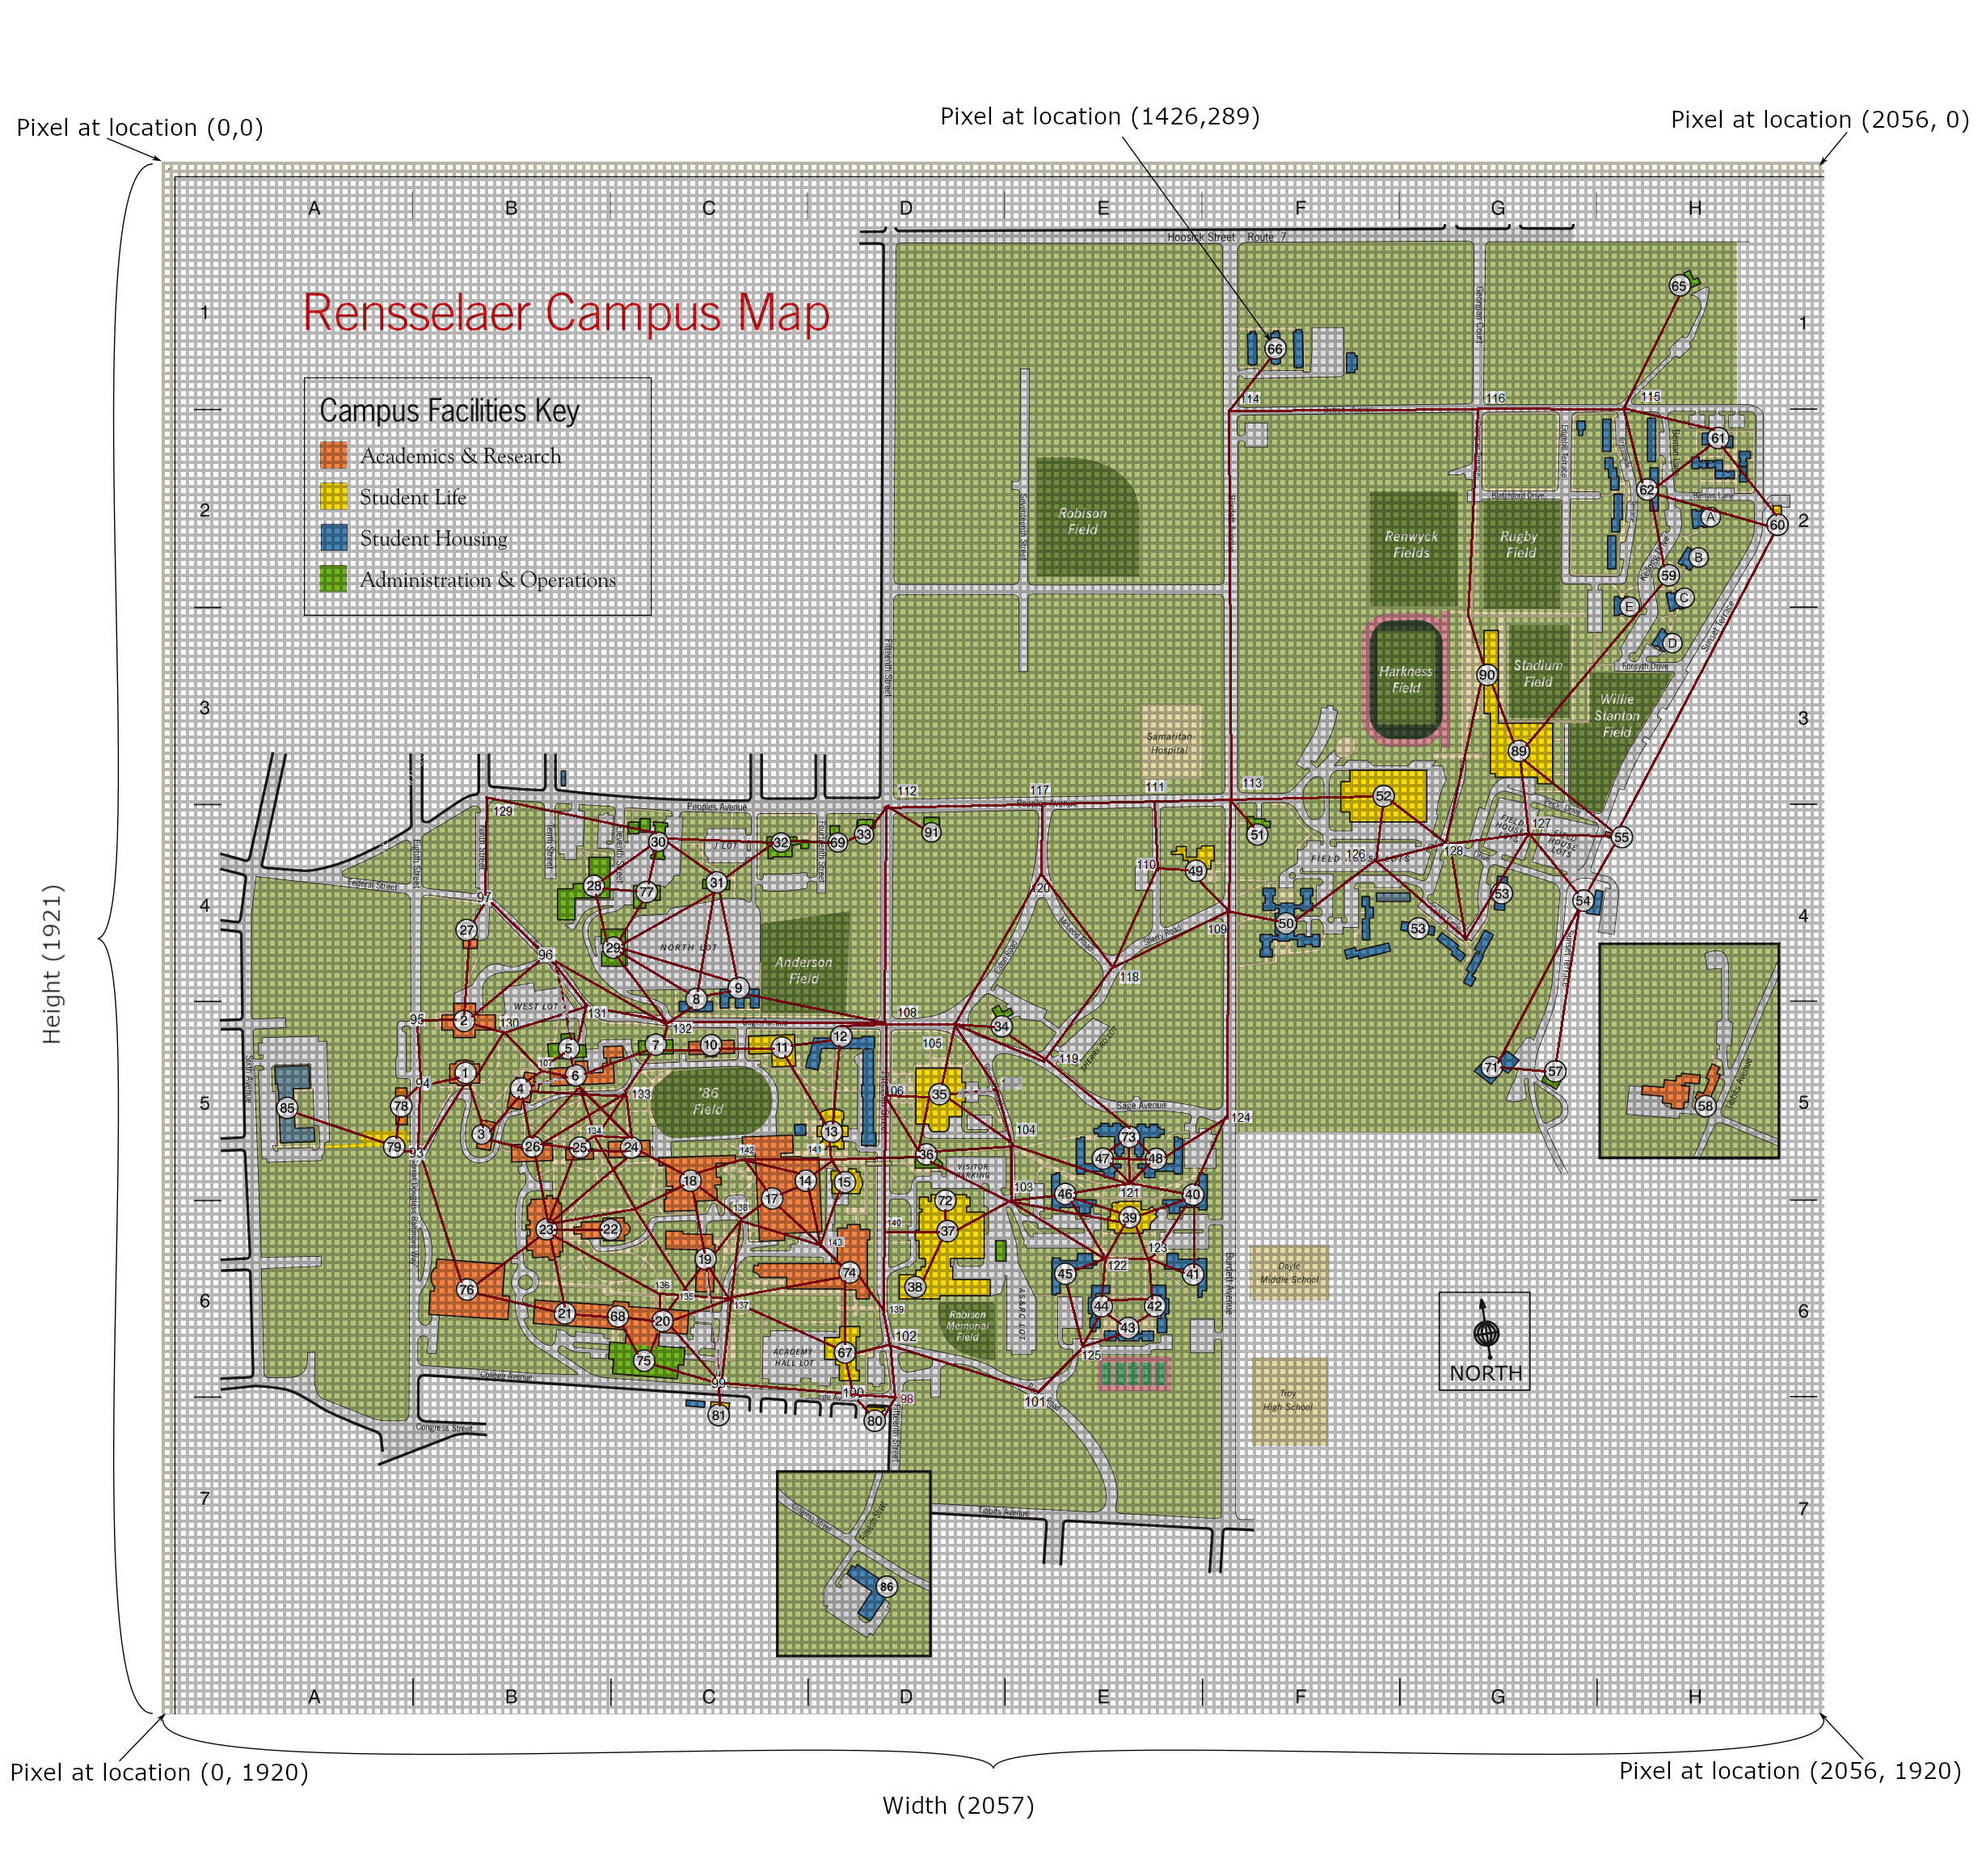
\includegraphics[scale=0.13]{RPI_campus_map_2010_extra_nodes_edges2_grid.png}
\newline
Another way of thinking about it is imagining that your campus map is in quadrant 4 of your coordinate plane instead of quadrant 1. In particular, this means that if you find any common math formulas involving trigonometric functions you might have to adjust them to the coordinate system used in this assignment by inverting the signs of y-axis parameters. Otherwise, you might get your computations wrong.

\section*{Problem 2: The Model}
\label{sec:Problem 2}

\noindent As described above, the model handles the data and contains the major logic and computation of your program. For this assignment, a key function of the model will be finding the shortest route between two building on campus. This can be accomplished by using Dijkstra's algorithm to find a shortest path in the graph, where edge weights represent the pathway length. Reuse the Dijkstra method by calling your Homework 6 code. \textcolor{red}{Do not copy and paste your Dijkstra code from Homework 6 into this homework.} Do not re-implement the Graph class in your Homework 7 code. Reuse the Graph class from Homework 4. Do not call methods of GraphWrapper from your Homework 7 code, use your Graph class directly. If you make changes to code from a previous homework, be aware that the code must still compile.

\section*{Problem 3: The Controller and View}
\label{sec:Problem 3}

\noindent In this homework, you will write a simple text interface. When the program is launched through the main method, it repeatedly prompts the user for one of the following one-character commands:

\begin{itemize}
\item \textit{b} lists all buildings (only buildings) in the form \texttt{name,id} in lexicographic (alphabetical) order of name.
\item \textit{r} prompts the user for the ids or names of two buildings (only buildings!) and prints directions for the shortest route between them.
\item \textit{q} quits the program. Note: this command should simply cause the main method to return. Calling \texttt{System.exit()} to terminate the program will break the tests.
\item \textit{m} prints a menu of all commands. Feel free to add functionality. Our tests cover only the functionality specified above.
\end{itemize}

\noindent When an unknown command is received the program prints the line:

\noindent \texttt{Unknown option}

\noindent Route directions start with:

\noindent \texttt{Path from \textit{Name 1} to \textit{Name 2}}:

\noindent where \textit{Name 1} and \textit{Name 2} are the full names of the two buildings specified by the user. Route directions are then printed with one line per pathway. Each line is indented with a single tab (\t) and reads:

\texttt{Walk direction to \textit{(Name 3)}}

\noindent where \textit{direction} is the direction of the pathway and \textit{Name 3} is the name of the building at the pathway destination. If the pathway destination is an intersection, print:

   \texttt{Walk direction to \textit{(Intersection id)}}

\noindent \textit{Direction} should be one of: North, NorthEast, East, SouthEast, South, SouthWest, West, or NorthWest. To determine the direction, compute the angle of the destination from direction north clockwise (e.g, angle of 90 degrees is East). This angle falls into one of eight 45 degree circle sectors corresponding to North, NorthEast, East, etc. as shown in the following diagram:

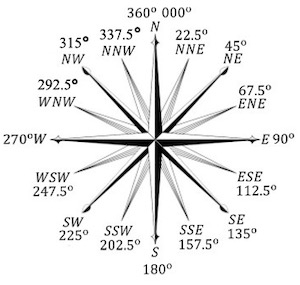
\includegraphics[scale=2]{compass.png}

\noindent For example, if the angle is in the sector [22.5, 67.5), the direction is NorthEast.

\noindent Finally, print the total distance in pixel units:

\noindent \texttt{Total distance: x pixel units.}

\noindent where x is the sum of the (non-rounded) distances of the individual route pathways.

\noindent The total distance should be rounded to three digits after the decimal point. As in Homework 6, we recommend the use of \href{https://docs.oracle.com/javase/8/docs/api/java/util/Formatter.html}{format strings.}

\noindent Finally, if one of the two buildings in a route is not in the dataset, the program prints the line:

\noindent \texttt{Unknown building: [Name]}

\noindent If neither building is in the dataset, the program prints the line twice, once for the first building and then for the second one. If there is no route between two buildings, your program should print:

\texttt{There is no path from Name 1 to Name 2.}

To help you with formatting your output correctly, we provide several sample files described in the table below. These files reflect the exact appearance of the console window after running the program, and include both user input and program output. If you run your program with the user input shown in the table, the state of the console should match sample file contents exactly (including whitespace). The sample files and the descriptions above, taken together, should completely specify the output format of your program.

\begin{center}
\begin{tabular}{ | m{5cm} | m{5cm}| m{5cm} | } 
  \hline
  \textbf{Description} & \textbf{Command(s) entered by the user} & \textbf{Sample file} \\ 
  \hline
  A list of all buildings. & \texttt{b \newline q} & \href{https://www.cs.rpi.edu/academics/courses/spring23/csci2600/Documents/sample_hw7_output_00.txt}{sample\_hw7\_output\_00.txt}\\ 
  \hline
  A path between two buildings. Buildings are given by their ids. & \texttt{r \newline 67 \newline 76 \newline q} & \href{https://www.cs.rpi.edu/academics/courses/spring23/csci2600/Documents/sample_hw7_output_01.txt}{sample\_hw7\_output\_01.txt} \\ 
  \hline
  A path between two buildings. Buildings are given by their names. & \texttt{r \newline EMPAC \newline Academy Hall \newline q} & \href{https://www.cs.rpi.edu/academics/courses/spring23/csci2600/Documents/sample_hw7_output_02.txt}{sample\_hw7\_output\_02.txt} \\
  \hline
  No path between two buildings. Buildings are given by their names/ids. & \texttt{r \newline LINAC Facility \newline 60 \newline q} & \href{https://www.cs.rpi.edu/academics/courses/spring23/csci2600/Documents/sample_hw7_output_03.txt}{sample\_hw7\_output\_03.txt} \\
  \hline
  One of the buildings is not found. & \texttt{r \newline 60 \newline cbis \newline q} & \href{https://www.cs.rpi.edu/academics/courses/spring23/csci2600/Documents/sample_hw7_output_04.txt}{sample\_hw7\_output\_04.txt} \\
  \hline
  Both buildings are not found. & \texttt{r \newline Louis Rubin Memorial Approach \newline 102 \newline q} & \href{https://www.cs.rpi.edu/academics/courses/spring23/csci2600/Documents//sample_hw7_output_05.txt}{sample\_hw7\_output\_05.txt} \\
  \hline
  A path from the building to itself. & \texttt{r \newline East Campus Athletic Village Arena \newline 89 \newline q} & \href{https://www.cs.rpi.edu/academics/courses/spring23/csci2600/Documents//sample_hw7_output_06.txt}{sample\_hw7\_output\_06.txt} \\
  \hline
  The menu of all commands. For this command, your output may be different from what is shown in the sample output file. & \texttt{m \newline q} & \href{https://www.cs.rpi.edu/academics/courses/spring23/csci2600/Documents//sample_hw7_output_07.txt}{sample\_hw7\_output\_07.txt} \\
  \hline
  An unknown command. & \texttt{a \newline q} & \href{https://www.cs.rpi.edu/academics/courses/spring23/csci2600/Documents//sample_hw7_output_08.txt}{sample\_hw7\_output\_08.txt} \\
  \hline
  \end{tabular}
  \end{center}

\begin{center}
  \begin{tabular}{ | m{5cm} | m{5cm}| m{5cm} | } 

  \hline
  Several commands in one session. & \texttt{a \newline m \newline r \newline 7 \newline 11 \newline r \newline 81 \newline 20 \newline b \newline r \newline Lally \newline Lally Hall \newline r \newline Troy Building \newline 11 \newline r \newline Troy Building \newline 87 Gymnasium \newline q} & \href{https://www.cs.rpi.edu/academics/courses/spring23/csci2600/Documents//sample_hw7_output_09.txt}{sample\_hw7\_output\_09.txt} \\
  \hline
  \end{tabular}
  \end{center}

\section*{Problem 4: Testing Your Solution}
\label{sec:Problem 4}

Unlike in previous assignments, the specification is based solely on the output of the complete application, as invoked through the \texttt{main} method. This means that your JUnit tests will be different from previous homework assignments.

\noindent We provide class \texttt{CampusPathsTest.java} as the starter code. The \texttt{runTest()} method takes as a parameter the name of the test files and then constructs three file names, one for input, one for expected output, and one for actual output. It temporarily points \texttt{System.in} to the input file and \texttt{System.out} to the actual output file while it runs your main program. The result is that commands are read from the input file and output is printed to the output file. For your tests to run, you simply need to add \texttt{@Test} methods that call \texttt{runTest()} with the appropriate argument. Also, you might have to edit the designated line in runTest to invoke your main() method.

\noindent You will specify the commands for your tests to run in \texttt{*.test} files. These files simply contain the input a user would have entered at the command line as the program was running. For each test, a corresponding \texttt{.expected} file should contain the output your program is expected to print if a user entered that input. Use JUnit to run the tests. \texttt{runTest()} compares the output in your \texttt{.out} file against the corresponding \texttt{.expected} file.

\noindent Reminder: if a test fails, it is often helpful to look at the \texttt{.out} file. These files are written to the \texttt{data/} directory. It might be easier to navigate through the file system using your system's file browser or the terminal, rather than in Eclipse.

\noindent We have provided one example test in \texttt{data}. Note that the \texttt{.expected} file only contains newlines printed by the program using \texttt{System.out.println()}.
\newpage

\noindent \textcolor{red}{It is important that your test data, i.e., \texttt{*.test} and \texttt{*.expected} files, are placed in directory \texttt{data/} and not in directory \texttt{src/test/java/hw7/}. If you place your test data under \texttt{test/} the Homework Server won't grab the files and will produce FileNotFound Exceptions.}

\noindent Additionally, you should write JUnit tests for every class that is not part of the view or controller. You may not need to write tests for the view and controller. One reason is that they should  have very little functionality — they act as glue between the UI (which is hard to test programmatically) and the model. Furthermore, end-to-end behavior of your application is tested through the specification tests. You may write additional tests for your view and controller if you feel there are important cases not covered by your specification tests, but avoid creating unnecessary work for yourself by duplicating tests. You must have at least three different path tests. The code coverage threshold will be set at 85\% for this assignment.

\section*{Reflection [0.5 points]}
Please answer the following questions in a file named \texttt{hw7\_reflection.pdf} in your \texttt{answers/} directory. Answer briefly, but in enough detail to help you improve your own practice via introspection and to enable the course staff to improve Principles of Software in the future.
\begin{enumerate}
\item In retrospect, what could you have done better to reduce the time you spent solving this assignment?
\item What could the Principles of Software staff have done better to improve your learning experience in this assignment?
\item What do you know now that you wish you had known before beginning the assignment?
\end{enumerate}

\section*{Collaboration[0.5 points]}
Please answer the following questions in a file named \texttt{hw7\_collaboration.pdf} in your \texttt{answers/} directory.

\noindent The standard \href{https://www.cs.rpi.edu/academics/courses/spring23/csci2600/Documents/syllabus_CSCI_2600_Spring_2023.pdf}{integrity policy} applies to this assignment.

\noindent State whether you collaborated with other students. If you did collaborate with other students, state their names and a brief description of how you collaborated.

\newpage

\noindent {\huge\textbf{\underline{Grade Breakdown}}}
\begin{itemize}
\item Quality of test suite, percent of your tests passed: 5 pts (auto-graded)
\item Quality of test suite, percent coverage: 5 pts (auto-graded)
\item Instructor tests: 16 pts (auto-graded)
\item Answers to MVC questions (\texttt{answers/hw7\_mvc.pdf}): 5 pts
\item Test data quality (\texttt{data/*.test} and \texttt{data/*.expected}): 3 pts
\item Code quality (\texttt{src/main/java/hw7/*.java}, Principles of Software specs, implementation of Observer/MVC and code reuse): 15 pts
\item Collaboration and reflection: 1 pt
\end{itemize}

\section*{Hints}
\label{sec:Hints}
\large{\textbf{Best Coding Practices}}

\noindent When designing classes, keep the single responsibility principle in mind. Avoid huge “god” classes.

\noindent Remember to practice good procedural decomposition: each method should be short and represent a single logical operation or common task. In particular, it can be tempting to implement your entire view and controller as one long method, but strive to keep each method short by factoring operations into small helper methods.

\noindent Store your data in appropriate types/classes. In particular, you should \textit{not} pack together data into a \texttt{String} and then later parse the \texttt{String} to extract the components.

\noindent Remember that your graph should be completely hidden within the model. Classes that depend on the model (namely, the view and controller) should have no idea that the data is stored in a graph, not even from the class documentation. If you decided later to switch to a different graph ADT or to do away with the graph altogether (for example, by making calls to the Google Maps API to find paths), you want to be able to change the model without affecting the view and controller, whose job has nothing to do with how the data is stored or computed.

\noindent As usual, include an abstraction function, representation invariant, and checkRep() in all classes that represent an ADT. If a class does not represent an ADT, place a comment that explicitly says so where the AF and RI would normally go. (For example, classes that contain only static methods and are never constructed usually do not represent an ADT.) You very well may find that you have more non-ADT classes on this assignment than in the past. Please come to office hours if you feel unsure about what counts as an ADT and what doesn't.
\newpage

\noindent \large{\textbf{Common Issues}}

\noindent Do not call \texttt{System.exit()} to terminate your program, as it will prevent your specification tests from passing.

\noindent If you use \texttt{Scanner} to read user input from \texttt{System.in}, be sure not to call both \texttt{next()} and \texttt{nextLine()} on the same \texttt{Scanner} object, as the \texttt{Scanner} may misbehave. In particular, some students have found that it causes their programs to work correctly at the console but not when they run their tests. Using \texttt{Scanner} is neither necessary nor required.

\noindent Floating-point precision and numeric comparisons. If you do arithmetic over floating-point values (\texttt{float, double}), then an exact \texttt{==} may not work as expected. Thus, when comparing computed floating-point values, you should use an approximate comparison, such as that the ratio between the values is very close to 1. However, in this assignment you may use \texttt{==} if you are comparing exact floating-point values that are read from a file, without doing arithmetic over them. Doing an approximate comparison is even wrong, since it would give someone reading the code the impression that you are computing approximate values.

\section*{What to Turn In}
You should commit and push the following files to Submitty. Don't forget to click "Grade My Repository" button on Submitty!
\begin{itemize}
\item \texttt{src/main/java/hw7/*.java}
\item \texttt{data/*.test}
\item \texttt{data/*.expected}
\item \texttt{src/test/java/hw7/*Test.java} \textit{[JUnit test classes you edit or create]}
\item \texttt{answers/hw7\_mvc.pdf}
\item \texttt{answers/hw7\_reflection.pdf}
\item \texttt{answers/hw7\_collaboration.pdf}
\end{itemize}

\section*{Errata}
Check the \href{https://submitty.cs.rpi.edu/courses/s23/csci2600/forum}{Submitty Discussion Forum} for possible errata or other relevant information.

\section*{Q \& A}
\noindent None yet.

\noindent Parts of this homework were copied from the University of Washington Software Design and Implementation class by Michael Ernst.

\end{document}

